\begin{figure}[p]\centering
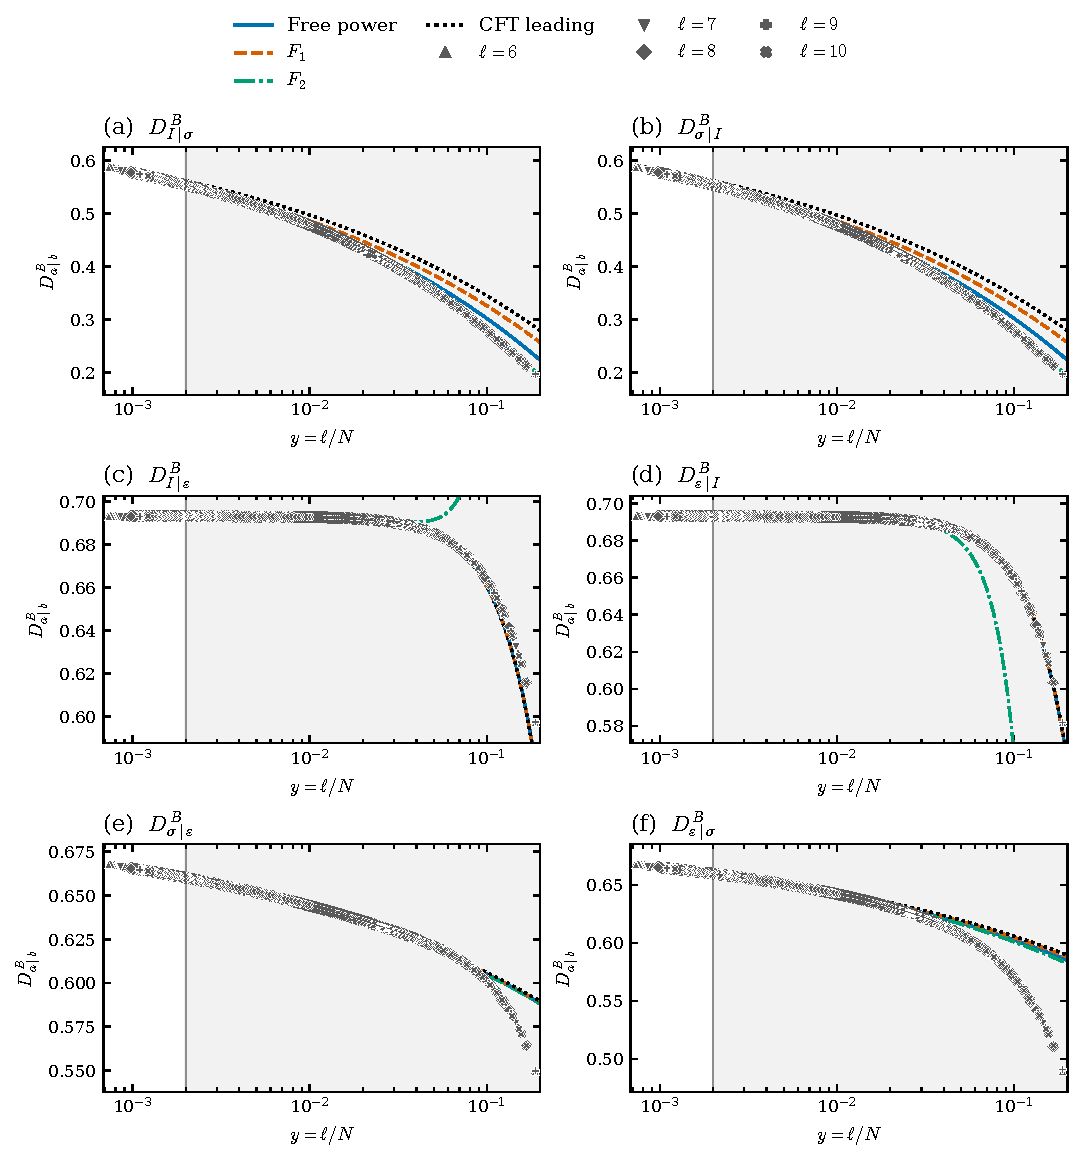
\includegraphics[width=.88\linewidth]{../figs/ising_large_entropy.pdf}
\caption{The ordinate is $D^B=\log2-\delta$, on a linear scale; tick labels give its value directly, without an additive offset. The fraction axis is logarithmic. Ising mixtures at $p=1/2$, $\ell=6,7,8,9,10$, and the chain-size set in Eq.~\eqref{eq:extended-grid}, with $32\leq N\leq8192$. There are 1645 displayed geometries per direction at $y\leq0.2$, of which 260 satisfy $y\leq0.002$ and enter every fit. Marker shape identifies $\ell$; the vertical boundary and gray shading mark the fitting cutoff and excluded data. The periodic Ising Hamiltonian is $H=-\sum_jX_jX_{j+1}-\sum_jZ_j$; primaries use exact fermionic covariances, including the odd Ramond ground state for $\sigma$. Natural logarithms apply. Added sizes use the direct entropy remainder in Sec.~\ref{sec:stable-entropy}, with support cutoff $10^{-15}$. Blue solid is the free-power fit (two fitted parameters), orange dashed is $F_1$ (one), green dash--dot is $F_2$ (two), and black dotted is the analytical CFT leading term (zero). Powers and amplitudes use Eqs.~\eqref{eq:fit} and \eqref{eq:complement-fit}; all coefficients include powers of $\pi$. Fits minimize unweighted squared residuals in $\delta$. These curves use \texttt{scaling\_fit\_summary.csv}. The identical fits in Tables~\ref{tab:ising-large-parameters} and \ref{tab:ising-large-metrics} also have per-pair full-range and fitting-window views in Sec.~\ref{sec:pair-large_ising}.}
\label{fig:ising-complement-entropy}
\end{figure}

\begin{figure}[p]\centering
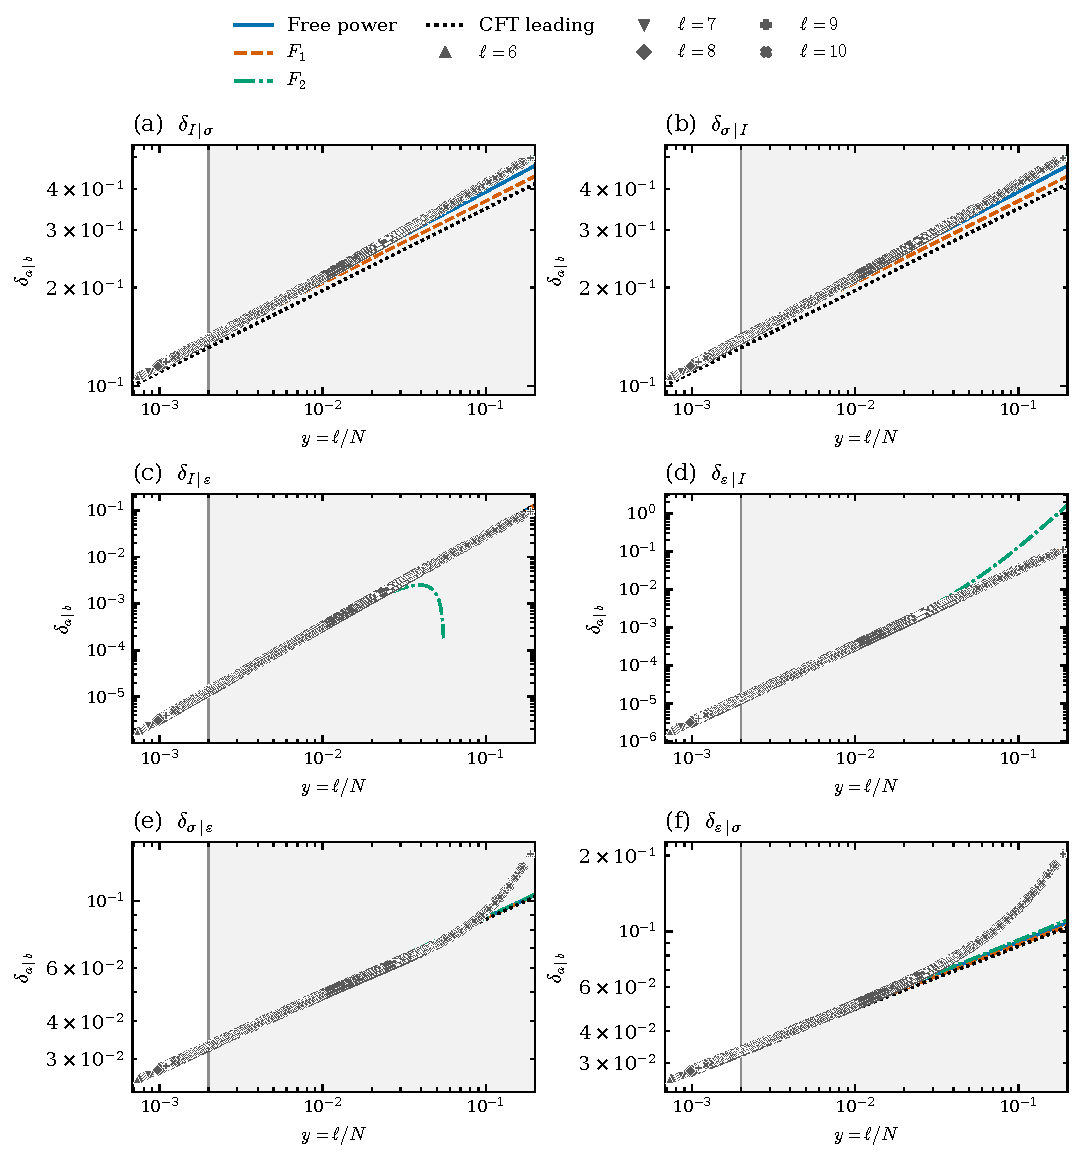
\includegraphics[width=.88\linewidth]{../figs/ising_large_value.pdf}
\caption{Both axes are logarithmic. Nonpositive values of an extrapolated truncated curve are omitted only from this logarithmic panel, while residual panels retain their predictions. Ising mixtures at $p=1/2$, $\ell=6,7,8,9,10$, and the chain-size set in Eq.~\eqref{eq:extended-grid}, with $32\leq N\leq8192$. There are 1645 displayed geometries per direction at $y\leq0.2$, of which 260 satisfy $y\leq0.002$ and enter every fit. Marker shape identifies $\ell$; the vertical boundary and gray shading mark the fitting cutoff and excluded data. The periodic Ising Hamiltonian is $H=-\sum_jX_jX_{j+1}-\sum_jZ_j$; primaries use exact fermionic covariances, including the odd Ramond ground state for $\sigma$. Natural logarithms apply. Added sizes use the direct entropy remainder in Sec.~\ref{sec:stable-entropy}, with support cutoff $10^{-15}$. Blue solid is the free-power fit (two fitted parameters), orange dashed is $F_1$ (one), green dash--dot is $F_2$ (two), and black dotted is the analytical CFT leading term (zero). Powers and amplitudes use Eqs.~\eqref{eq:fit} and \eqref{eq:complement-fit}; all coefficients include powers of $\pi$. Fits minimize unweighted squared residuals in $\delta$. These curves use \texttt{scaling\_fit\_summary.csv}. The identical fits in Tables~\ref{tab:ising-large-parameters} and \ref{tab:ising-large-metrics} also have per-pair full-range and fitting-window views in Sec.~\ref{sec:pair-large_ising}.}
\label{fig:ising-complement-deficit}
\end{figure}

\begin{figure}[p]\centering
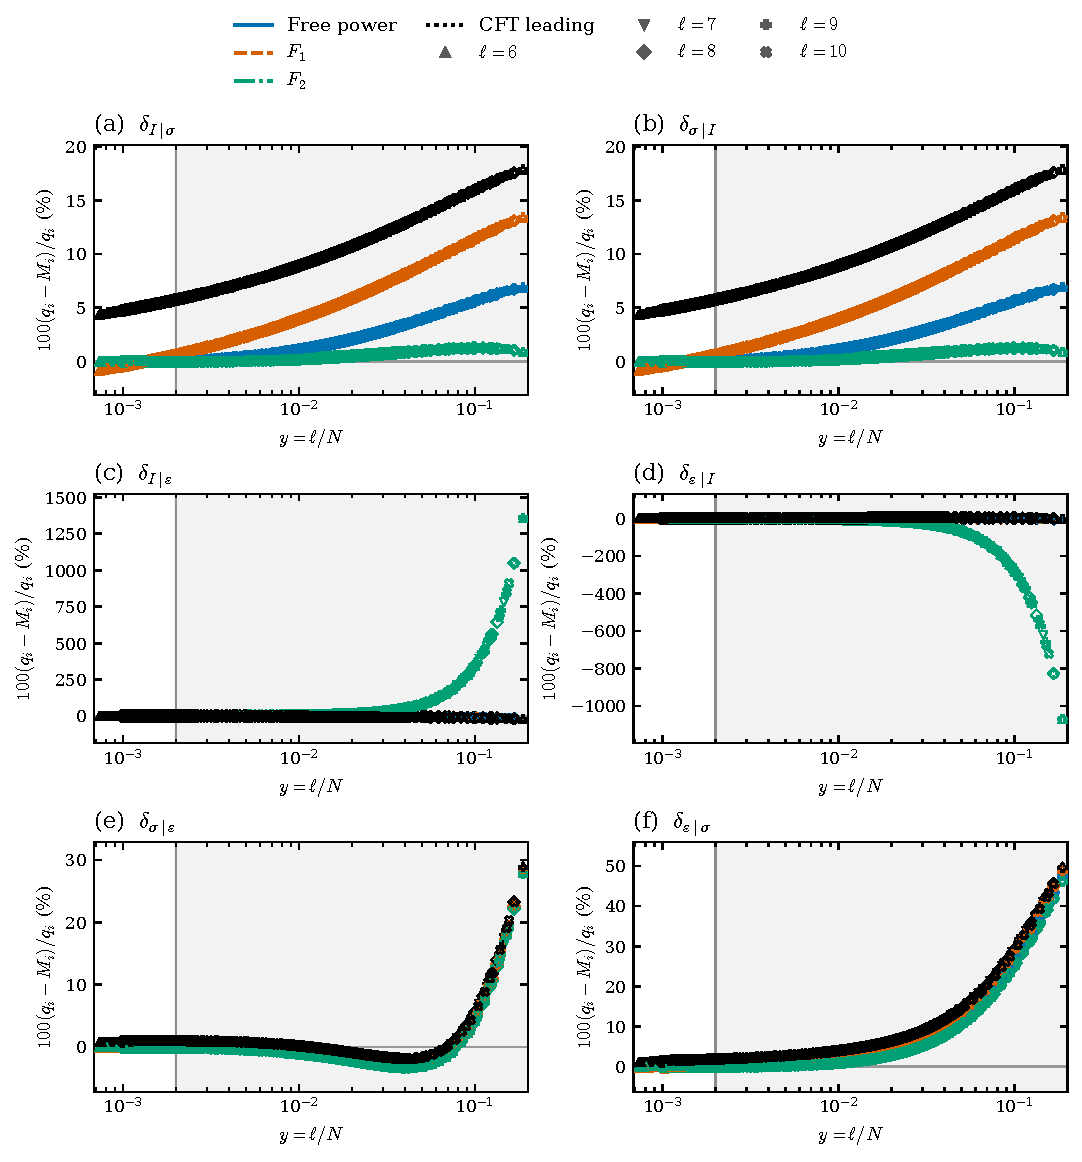
\includegraphics[width=.88\linewidth]{../figs/ising_large_residual.pdf}
\caption{The ordinate is $100(q_i-M_i)/q_i$ percent, with $q_i=D^A_i$ for a small interval and $q_i=\delta_i$ for a large interval; the horizontal zero line aids comparison. All four models have residual markers, colored as their curves. The residual ordinate is linear; the fraction axis is logarithmic. Ising mixtures at $p=1/2$, $\ell=6,7,8,9,10$, and the chain-size set in Eq.~\eqref{eq:extended-grid}, with $32\leq N\leq8192$. There are 1645 displayed geometries per direction at $y\leq0.2$, of which 260 satisfy $y\leq0.002$ and enter every fit. Marker shape identifies $\ell$; the vertical boundary and gray shading mark the fitting cutoff and excluded data. The periodic Ising Hamiltonian is $H=-\sum_jX_jX_{j+1}-\sum_jZ_j$; primaries use exact fermionic covariances, including the odd Ramond ground state for $\sigma$. Natural logarithms apply. Added sizes use the direct entropy remainder in Sec.~\ref{sec:stable-entropy}, with support cutoff $10^{-15}$. Blue solid is the free-power fit (two fitted parameters), orange dashed is $F_1$ (one), green dash--dot is $F_2$ (two), and black dotted is the analytical CFT leading term (zero). Powers and amplitudes use Eqs.~\eqref{eq:fit} and \eqref{eq:complement-fit}; all coefficients include powers of $\pi$. Fits minimize unweighted squared residuals in $\delta$. These curves use \texttt{scaling\_fit\_summary.csv}. The identical fits in Tables~\ref{tab:ising-large-parameters} and \ref{tab:ising-large-metrics} also have per-pair full-range and fitting-window views in Sec.~\ref{sec:pair-large_ising}.}
\label{fig:ising-complement-residuals}
\end{figure}

\begin{figure}[p]\centering
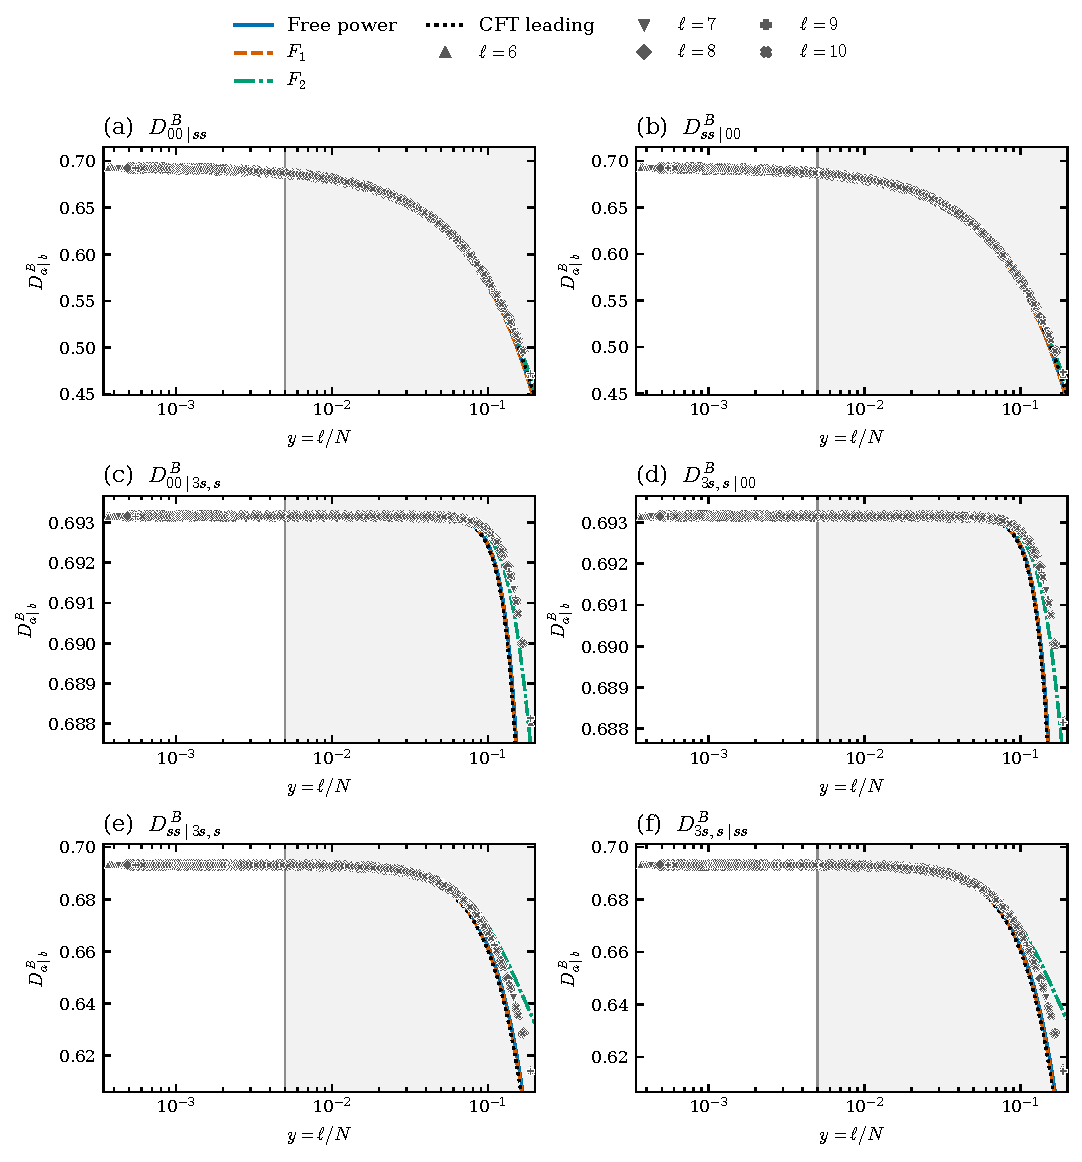
\includegraphics[width=.88\linewidth]{../figs/boson_large_entropy.pdf}
\caption{The ordinate is $D^B=\log2-\delta$, on a linear scale; tick labels give its value directly, without an additive offset. The fraction axis is logarithmic. Compact-boson mixtures at $p=1/2$, $\ell=6,7,8,9,10$, and the chain-size set in Eq.~\eqref{eq:extended-grid}, with $32\leq N\leq16384$. There are 625 displayed geometries per direction at $y\leq0.2$, of which 317 satisfy $y\leq0.005$ and enter every fit. Marker shape identifies $\ell$; the vertical boundary and gray shading mark the fitting cutoff and excluded data. The boson uses $s=1/\sqrt2$, $q=2$, charge codes $(0,0),(1,1),(3,1)$, $z_j=e^{2\pi i j/N}$, $w_1=0$, and $W=10^8$; moment algebra uses 100 digits through $N=256$ and 120 digits at the added sizes. Natural logarithms apply. Added sizes use the direct entropy remainder in Sec.~\ref{sec:stable-entropy}, with support cutoff $10^{-15}$. Blue solid is the free-power fit (two fitted parameters), orange dashed is $F_1$ (one), green dash--dot is $F_2$ (two), and black dotted is the analytical CFT leading term (zero). Powers and amplitudes use Eqs.~\eqref{eq:fit} and \eqref{eq:complement-fit}; all coefficients include powers of $\pi$. Fits minimize unweighted squared residuals in $\delta$. These curves use \texttt{scaling\_fit\_summary.csv}. The identical fits in Tables~\ref{tab:boson-large-parameters} and \ref{tab:boson-large-metrics} also have per-pair full-range and fitting-window views in Sec.~\ref{sec:pair-large_boson}.}
\label{fig:boson-complement-entropy}
\end{figure}

\begin{figure}[p]\centering
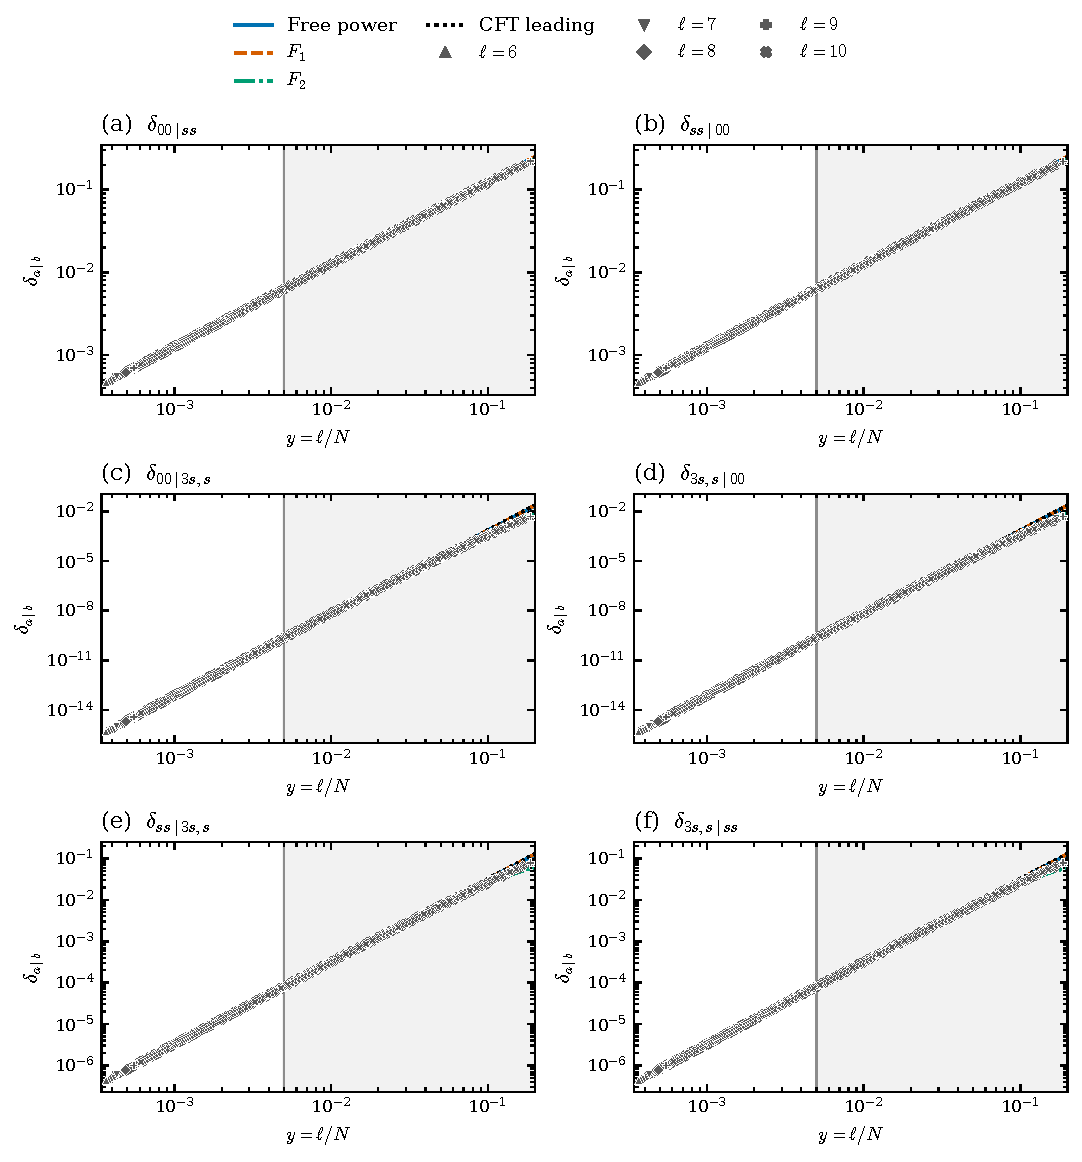
\includegraphics[width=.88\linewidth]{../figs/boson_large_value.pdf}
\caption{Both axes are logarithmic. Nonpositive values of an extrapolated truncated curve are omitted only from this logarithmic panel, while residual panels retain their predictions. Compact-boson mixtures at $p=1/2$, $\ell=6,7,8,9,10$, and the chain-size set in Eq.~\eqref{eq:extended-grid}, with $32\leq N\leq16384$. There are 625 displayed geometries per direction at $y\leq0.2$, of which 317 satisfy $y\leq0.005$ and enter every fit. Marker shape identifies $\ell$; the vertical boundary and gray shading mark the fitting cutoff and excluded data. The boson uses $s=1/\sqrt2$, $q=2$, charge codes $(0,0),(1,1),(3,1)$, $z_j=e^{2\pi i j/N}$, $w_1=0$, and $W=10^8$; moment algebra uses 100 digits through $N=256$ and 120 digits at the added sizes. Natural logarithms apply. Added sizes use the direct entropy remainder in Sec.~\ref{sec:stable-entropy}, with support cutoff $10^{-15}$. Blue solid is the free-power fit (two fitted parameters), orange dashed is $F_1$ (one), green dash--dot is $F_2$ (two), and black dotted is the analytical CFT leading term (zero). Powers and amplitudes use Eqs.~\eqref{eq:fit} and \eqref{eq:complement-fit}; all coefficients include powers of $\pi$. Fits minimize unweighted squared residuals in $\delta$. These curves use \texttt{scaling\_fit\_summary.csv}. The identical fits in Tables~\ref{tab:boson-large-parameters} and \ref{tab:boson-large-metrics} also have per-pair full-range and fitting-window views in Sec.~\ref{sec:pair-large_boson}.}
\label{fig:boson-complement-deficit}
\end{figure}

\begin{figure}[p]\centering
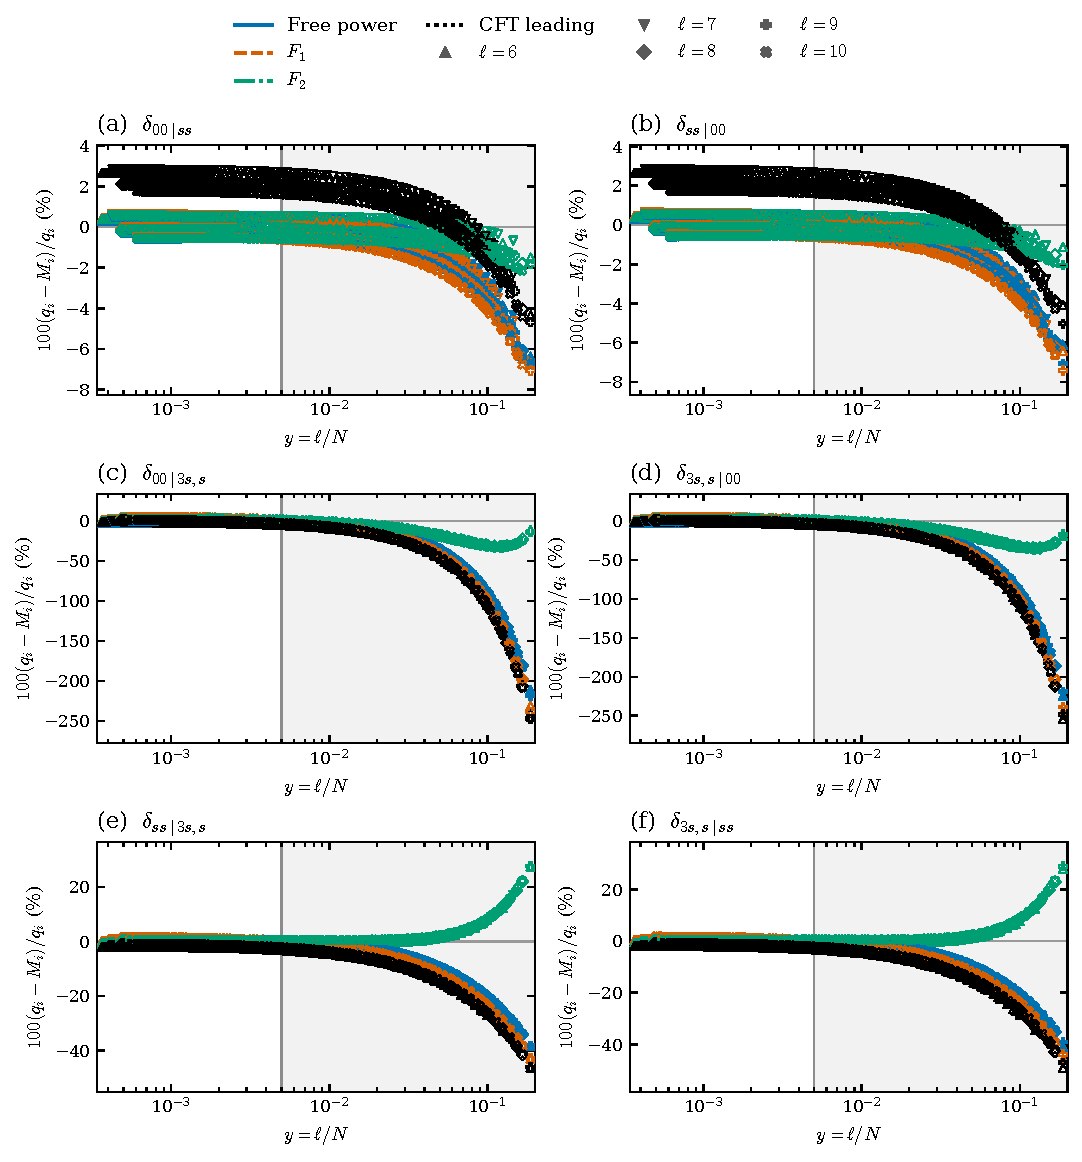
\includegraphics[width=.88\linewidth]{../figs/boson_large_residual.pdf}
\caption{The ordinate is $100(q_i-M_i)/q_i$ percent, with $q_i=D^A_i$ for a small interval and $q_i=\delta_i$ for a large interval; the horizontal zero line aids comparison. All four models have residual markers, colored as their curves. The residual ordinate is linear; the fraction axis is logarithmic. Compact-boson mixtures at $p=1/2$, $\ell=6,7,8,9,10$, and the chain-size set in Eq.~\eqref{eq:extended-grid}, with $32\leq N\leq16384$. There are 625 displayed geometries per direction at $y\leq0.2$, of which 317 satisfy $y\leq0.005$ and enter every fit. Marker shape identifies $\ell$; the vertical boundary and gray shading mark the fitting cutoff and excluded data. The boson uses $s=1/\sqrt2$, $q=2$, charge codes $(0,0),(1,1),(3,1)$, $z_j=e^{2\pi i j/N}$, $w_1=0$, and $W=10^8$; moment algebra uses 100 digits through $N=256$ and 120 digits at the added sizes. Natural logarithms apply. Added sizes use the direct entropy remainder in Sec.~\ref{sec:stable-entropy}, with support cutoff $10^{-15}$. Blue solid is the free-power fit (two fitted parameters), orange dashed is $F_1$ (one), green dash--dot is $F_2$ (two), and black dotted is the analytical CFT leading term (zero). Powers and amplitudes use Eqs.~\eqref{eq:fit} and \eqref{eq:complement-fit}; all coefficients include powers of $\pi$. Fits minimize unweighted squared residuals in $\delta$. These curves use \texttt{scaling\_fit\_summary.csv}. The identical fits in Tables~\ref{tab:boson-large-parameters} and \ref{tab:boson-large-metrics} also have per-pair full-range and fitting-window views in Sec.~\ref{sec:pair-large_boson}.}
\label{fig:boson-complement-residuals}
\end{figure}
